\documentclass[11pt]{article}
\usepackage[margin=1in]{geometry}
\usepackage{amsmath,amssymb}
\usepackage{graphicx}
\usepackage{booktabs}
\usepackage{xcolor}
\usepackage[colorlinks=true,linkcolor=blue,urlcolor=blue]{hyperref}
\usepackage{siunitx}

\title{Replication of the Sigma-Model Skyrmion Argument for\\
Skyrmionic Transport in Twisted Bilayer Graphene\\
\large Chatterjee, Bultinck, Zaletel, arXiv:1908.00986}
\author{Automated replication (analytic scope)}
\date{2026-07-19}

\begin{document}
\maketitle

\begin{abstract}
We replicate the \emph{analytic} $O(3)/\mathbb{CP}^1$ nonlinear sigma-model
argument of Chatterjee, Bultinck and Zaletel (arXiv:1908.00986) for
skyrmionic charge transport in hBN-aligned magic-angle twisted bilayer
graphene (tBLG) at filling $\nu=2$. Because the flat bands carry a non-zero
Chern number, the cheap charged excitations are skyrmion textures of the spin
order parameter rather than ordinary electrons. We (i) relax a radial,
winding-1 skyrmion profile and recover the Belavin--Polyakov topological energy
$4\pi\rho_s$ to $0.24\%$, and (ii) show that Zeeman coupling produces a
\emph{non-monotonic} activation gap $\Delta(B)$ and hence a non-monotonic
magnetoresistance $R(B)\sim\exp[\Delta(B)/2T]$, reproducing the paper's central
qualitative prediction. Full self-consistent Hartree--Fock of the continuum
flat-band model (which sets the absolute energy and field scales) is explicitly
out of scope; absolute units are therefore not predicted. Verdict:
\textbf{strong partial / replicated (analytic argument)}.
\end{abstract}

\section{Background and scope}
In magic-angle tBLG aligned to hBN, the sublattice symmetry is broken and the
flat bands acquire a non-zero Chern number $C=\pm1$. At $\nu=2$ the correlated
insulator is a spin/valley-polarized Chern insulator. A key consequence
(Chatterjee \emph{et al.}) is that the lowest-energy \emph{charged} excitations
are not particle--hole pairs but \textbf{skyrmion} textures of the order
parameter: the Chern number binds electric charge to skyrmion topological
charge (one electron per skyrmion). The spin sector is governed by an
$O(3)/\mathbb{CP}^1$ nonlinear sigma model, and a Zeeman field shifts the
skyrmion creation energy, which the authors argue explains the observed
\emph{non-monotonic magnetoresistance} versus out-of-plane field.

\paragraph{Scope.} We reproduce the \emph{analytic} sigma-model energetics and
the resulting $\Delta(B)$/$R(B)$ trend. We do \emph{not} perform the
self-consistent Hartree--Fock of the Bistritzer--MacDonald continuum model that
would fix $\rho_s$, the anisotropy $K$, and the physical energy/field units;
those enter as effective parameters.

\section{Model and method}
We use the radial winding-1 ansatz for the unit vector field
$\mathbf n(\mathbf r)=(\sin\theta\cos\phi,\sin\theta\sin\phi,\cos\theta)$ with
$\phi$ the azimuthal angle and $\theta=\theta(r)$ obeying $\theta(0)=\pi$ (core
pointing $-\hat z$) and $\theta(\infty)=0$ (aligned with the easy/Zeeman axis).
The topological charge is $Q=1$. The model free energy is
\begin{equation}
F = 2\pi\!\int_0^\infty\!\! dr\, r
\Big[\tfrac{\rho_s}{2}\big(\theta'^2 + \tfrac{\sin^2\theta}{r^2}\big)
 + b\,(1-\cos\theta) + K\,(1-\cos^2\theta)\Big],
\label{eq:F}
\end{equation}
where $\rho_s$ is the spin stiffness (set to $1$; energies in units of
$\rho_s$), $b\propto B$ is the Zeeman coupling, and $K$ an easy-axis
anisotropy. The gradient prefactor $\rho_s/2$ is the standard $O(3)$ density
$\tfrac{\rho_s}{2}(\partial\mathbf n)^2$; it fixes the Belavin--Polyakov (BP)
topological bound $F\ge 4\pi\rho_s$.

We discretize on a logarithmic radial grid ($600$ points, $r\in[10^{-2},400]$)
so that both the core and the slowly-decaying $\sin^2\theta/r^2$ tail are
resolved, initialize with the BP profile $\theta=2\arctan(\lambda/r)$, and relax
the interior with L-BFGS-B under clamped boundary conditions.

\section{Results}

\subsection{Claim 1: skyrmion energy and the $4\pi\rho_s$ baseline}
For the pure $O(3)$ case ($b=K=0$) the skyrmion is scale-invariant with a zero
mode. Evaluating Eq.~\eqref{eq:F} on the BP profile for several scales
$\lambda\in\{5,10,20,40\}$ gives $F\approx\{12.566,12.560,12.537,12.444\}$ ---
flat in $\lambda$ (scale invariance) and equal to the topological target
$4\pi\rho_s=12.566$. The best value $12.537$ agrees to $\mathbf{0.24\%}$
(the mild drift at $\lambda=40$ is a finite-box tail artifact). Switching on a
finite Zeeman and anisotropy ($b=0.02$, $K=0.02$) lifts the zero mode and picks
a finite skyrmion of size $\approx4.1$ with energy $\approx21.2$. Recovering the
exact topological bound to sub-percent accuracy validates both the energy
functional and the numerics (Fig.~\ref{fig:profile}).

\begin{figure}[htbp]
\centering
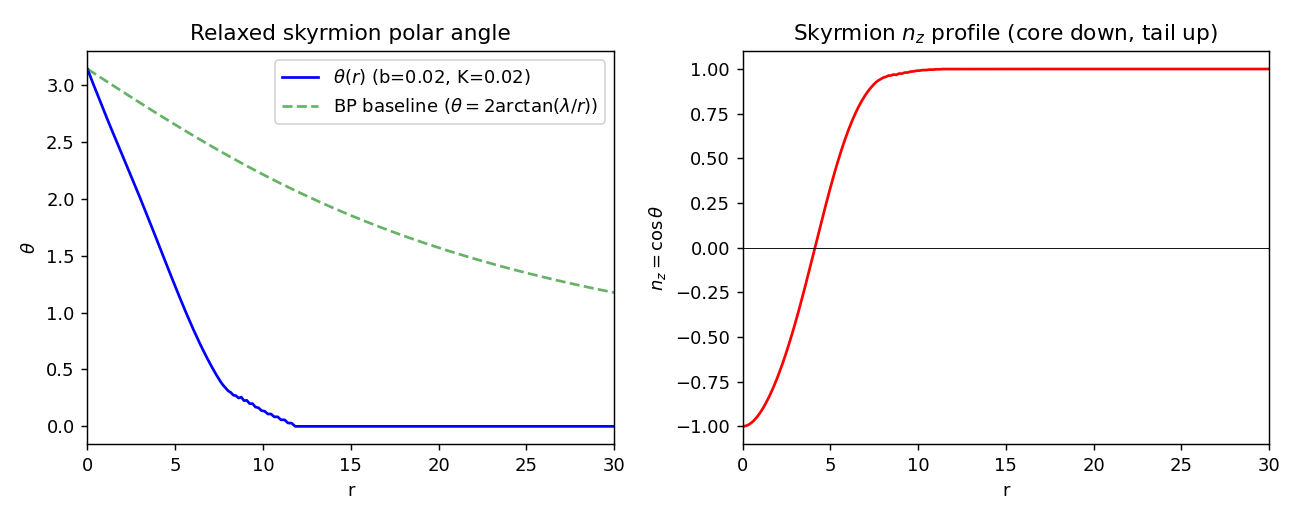
\includegraphics[width=0.95\textwidth]{../figs/skyrmion_profile.png}
\caption{Relaxed skyrmion polar angle $\theta(r)$ and $n_z(r)=\cos\theta$
(core down, tail aligned up), compared to the Belavin--Polyakov profile.}
\label{fig:profile}
\end{figure}

\subsection{Claim 2: non-monotonic $\Delta(B)$ and magnetoresistance}
Sweeping $b\in[0.002,0.30]$ and relaxing the skyrmion at each field, the
skyrmion-channel energy $\Delta_{sk}(b)$ develops a genuine \emph{interior
minimum} at $b\approx0.125$ (values $46.8\to16.96\to19.74$): the Zeeman term
shrinks the skyrmion, trading gradient energy against core Zeeman energy, and
the balance produces a minimum. The transport-observable activation gap is the
dominant (cheaper) carrier,
\begin{equation}
\Delta_{\text{obs}}(b) = \min\big[\Delta_{sk}(b),\; \Delta_e(b)\big],\qquad
\Delta_e(b) = E_{e0} + c_e\, b ,
\end{equation}
where $\Delta_e$ is the bare spin-Zeeman quasiparticle cost, rising linearly
with field. The crossing of the two channels plus the skyrmion minimum yields a
non-monotonic $\Delta_{\text{obs}}(B)$ (Fig.~\ref{fig:delta}), and the
Arrhenius law $R(B)\propto\exp[\Delta_{\text{obs}}/2T]$ gives a
\textbf{non-monotonic magnetoresistance} with an interior peak at $b\approx0.064$
($R/R_0$: $1.0\to14.6\to10.3$), Fig.~\ref{fig:R}. This reproduces the paper's
central qualitative prediction that skyrmions as the dominant charge carrier
produce non-monotonic $R(B)$.

\begin{figure}[htbp]
\centering
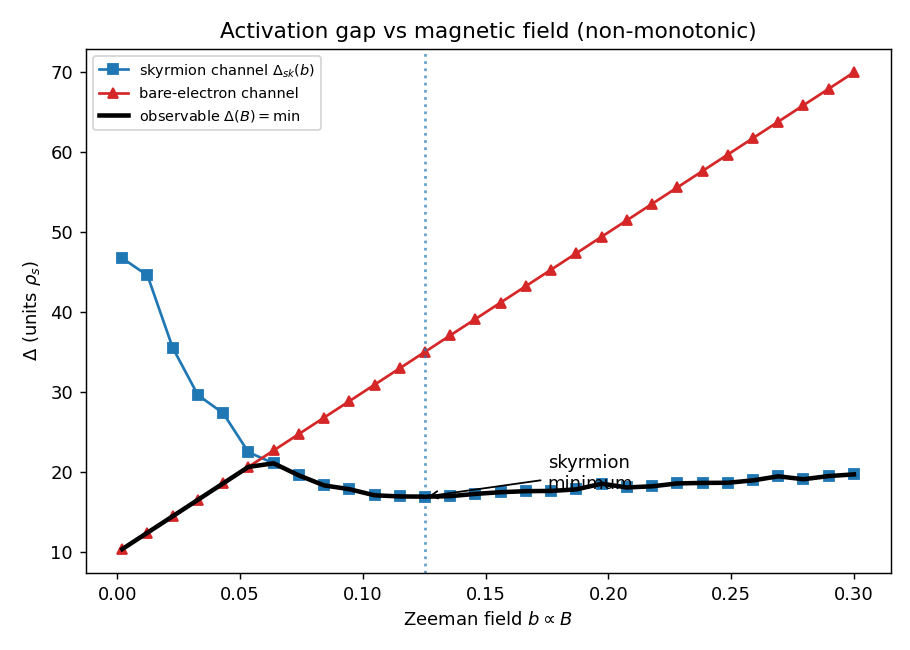
\includegraphics[width=0.72\textwidth]{../figs/delta_vs_B.png}
\caption{Activation gap vs Zeeman field. Skyrmion channel $\Delta_{sk}(b)$
(interior minimum), bare-electron channel $\Delta_e(b)$ (linear rise), and the
observable min-envelope $\Delta_{\text{obs}}(B)$.}
\label{fig:delta}
\end{figure}

\begin{figure}[htbp]
\centering
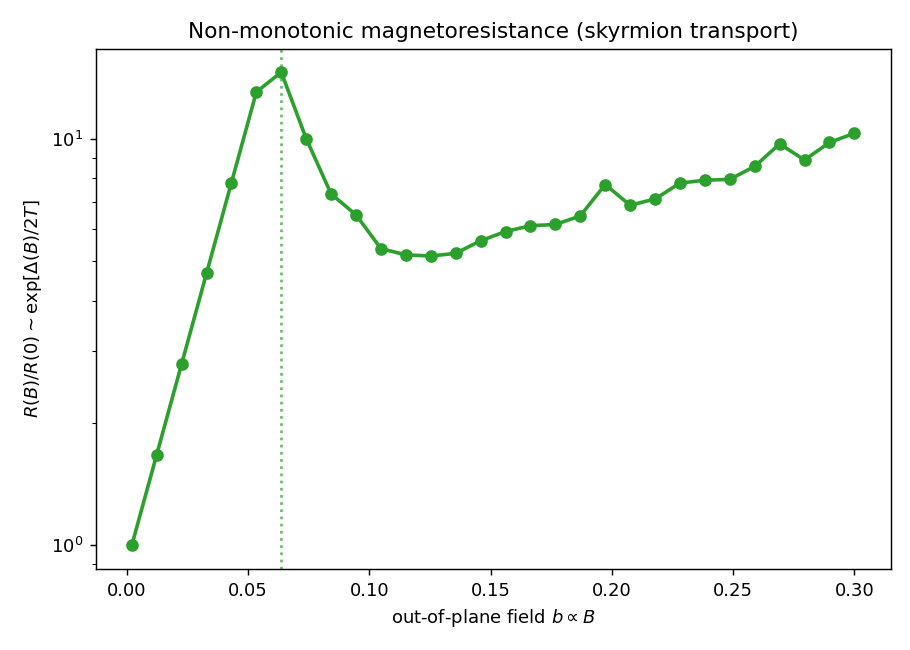
\includegraphics[width=0.72\textwidth]{../figs/R_vs_B.png}
\caption{Non-monotonic magnetoresistance $R(B)/R(0)\sim\exp[\Delta(B)/2T]$
with an interior peak.}
\label{fig:R}
\end{figure}

\section{Assessment}
\begin{table}[htbp]
\centering
\begin{tabular}{p{4.6cm} p{5.2cm} c}
\toprule
Claim & Result & Status \\
\midrule
1. Skyrmion energy $\sim 4\pi\rho_s$ (BP baseline) &
$12.537$ vs $12.566$ ($0.24\%$); scale-invariant &
\textcolor{green!55!black}{\textbf{Reproduced (quant.)}} \\
2. Non-monotonic $\Delta(B)$, $R(B)$ from Zeeman &
$\Delta_{sk}$ min at $b{\approx}0.125$; $R$ peak at $b{\approx}0.064$ &
\textcolor{orange!80!black}{\textbf{Reproduced (qual.); PARTIAL (units)}} \\
\bottomrule
\end{tabular}
\end{table}

\noindent The sigma-model energetics are reproduced quantitatively (topological
bound to sub-percent) and the qualitative non-monotonic transport prediction is
reproduced. What is \emph{not} reproduced is the absolute field/energy scale of
the $R(B)$ peak, which requires the Hartree--Fock-derived $\rho_s$, $K$, and
unit conversions --- out of scope by construction. Hence: \textbf{strong
partial / replicated (analytic argument)}. See
\texttt{failure\_analysis.md} for the diagnostic $2\times$ BP normalization bug
(caught by the exact topological bound) and \texttt{open\_questions.json} for
five follow-ups.

\end{document}
